% 経路追従モジュールの詳細図．paper.tex から \input して使う．
% 観測画像と深度マップは未学習環境 m の実データおよび UniDepth の実出力．
% CARE の補正を表す top-down の模式図は例示．
\begin{tikzpicture}[
    font=\normalsize,
    x=0.85cm,
    blk/.style={draw, align=center, minimum height=8mm, minimum width=16mm,
                inner xsep=2pt},
    val/.style={draw, align=center, minimum height=6.5mm, minimum width=9mm},
    pic/.style={draw, inner sep=0pt},
    grp/.style={draw, dashed, gray},
    frz/.style={fill=cyan!12},
    lbl/.style={font=\small, inner sep=1.5pt},
    ar/.style={-{Latex[length=1.6mm]}, thin},
]
% ---- 観測 ----------------------------------------------------------------
\node[pic] (o3) at (0,0) {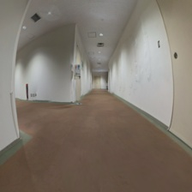
\includegraphics[width=15mm]{images/pf_obs3.png}};
\node[pic] (o2) at (-0.1,0.1) {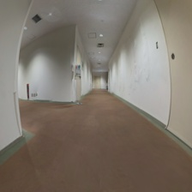
\includegraphics[width=15mm]{images/pf_obs2.png}};
\node[pic] (o1) at (-0.2,0.2) {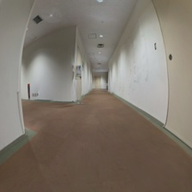
\includegraphics[width=15mm]{images/pf_obs1.png}};
\node[lbl, below=0.5mm of o3, align=center] {RGB images\\$4$ frames};

% ---- NoMaD 本体 ----------------------------------------------------------
\node[blk, frz] (enc) at (3.9,0) {Image encoder\\\small EfficientNet\text{-}B0, \frozen};
\node[blk, frz] (trn) at (7.8,0) {Transformer\\\small \frozen};
\node[circle, draw, inner sep=1.2pt] (sum) at (10.2,0) {$+$};
\node[blk, minimum width=21mm] (dif) at (13.5,0)
      {Diffusion policy\\\small $8$ waypoints};

% ---- 目標方向（本研究で追加）---------------------------------------------
% 直進・左折・右折のアイコン．この例では左折を与えているため，左折を強調する．
\def\diricon#1#2{\tikz[baseline=0, line width=1pt, rounded corners=1.1mm]
    \draw[-{Latex[length=1.8mm, width=2.1mm]}, #1] #2;}
\def\diricons{\diricon{}{(0,0) -- (0,4.2mm)}\quad
    \diricon{red, line width=1.8pt}{(0,0) |- (-2.9mm,3mm)}\quad
    \diricon{}{(0,0) |- (2.9mm,3mm)}}
\node[blk, fill=black!8, minimum width=21mm] (cmd) at (3.6,-1.7) {Target direction\\[0.5mm]\diricons};
\node[blk, fill=black!8] (den) at (7.8,-1.7) {Direction encoder\\\small 3\text{-}layer MLP};

% ---- 深度・障害物 --------------------------------------------------------
\node[blk, minimum width=18mm] (udp) at (3.6,-3.7) {\UniDepth};
\node[pic] (dep) at (6.6,-3.7) {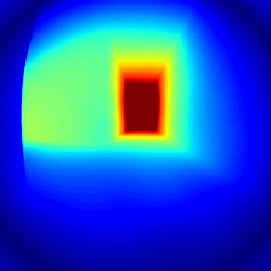
\includegraphics[width=13mm]{images/pf_depth_cmap.png}};
\node[pic] (bev) at (9.6,-3.7) {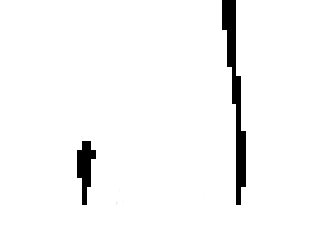
\includegraphics[height=13mm]{images/pf_bev_cc_noarrow.png}};
\draw (bev.south west) rectangle (bev.north east);
\node[lbl, below=0.5mm of bev] {BEV};

% ---- CARE ----------------------------------------------------------------
\node[blk] (care) at (13.5,-3.7) {\CARE};
\node[val] (vw)  at (17.95,-3.7) {$(v,\omega)$};

% ---- CARE による補正の模式図（例示）--------------------------------------
% 背景は BEV と同じ画像（幅 1.9 の座標系に合わせて軌道を重ねる）．
% scale で画像幅 2.4cm に合わせて座標系ごと拡大する．
\begin{scope}[shift={(16.75,-2.4)}, x=1cm, y=1cm, scale=2.4/1.9]
  \node[anchor=south west, inner sep=0pt] at (0,0)
        {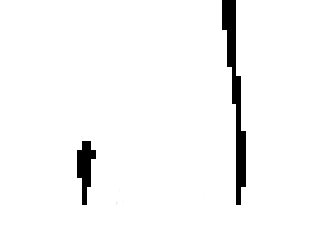
\includegraphics[width=2.4cm]{images/pf_bev_cc_noarrow.png}};
  \draw (0,0) rectangle (1.9,1.365);
  \draw[densely dashed, gray, thick] (0.96,0.17)
        .. controls (0.96,0.45) and (0.8,0.62) .. (0.3,0.68)
        node[lbl, below, inner sep=1.5pt] {$p_k$};
  \draw[thick] (0.96,0.17)
        .. controls (0.96,0.7) and (0.8,0.95) .. (0.2,1.0)
        node[lbl, pos=0.8, above, inner sep=1.5pt] {$p'_k$};
  \node[lbl, anchor=north] (toplab) at (0.95,0) {example};
\end{scope}
\coordinate (topsw) at (16.75,-2.4);

% ---- 結線 ----------------------------------------------------------------
\draw[ar] (o3) -- (enc);
\draw[ar] (enc) -- (trn);
\draw[ar] (trn) -- (sum);
\draw[ar] (sum) -- (dif);
\draw[ar] (cmd) -- (den);
\draw[ar] (den.east) -| (sum.south);
\draw[ar] (o1.west) -- ++(-0.35,0) |- (udp.west);
\draw[ar] (udp) -- (dep);
\draw[ar] (dep) -- (bev);
\draw[ar] (dif.south -| care.north) -- (care.north);
\draw[ar] (bev) -- (care);
\draw[ar] (care) -- (vw);
\draw[black!60, densely dashed, thick] (care.north east) -- (topsw);


% ---- 枠 ------------------------------------------------------------------
\begin{scope}[on background layer]
  \node[grp, fit=(enc)(dif)(cmd)(den), inner sep=3mm] (gn) {};
\end{scope}
\node[lbl, anchor=north west, fill=white, inner xsep=2pt]
      at ([xshift=2mm,yshift=0.2mm]gn.north west) {Direction\text{-}conditioned \NoMaD};
\end{tikzpicture}
